\setcounter{section}{1}

\section{Lecture 2:Jan 22}

\subsection*{Last time}
\begin{itemize}
\item Introduction
\item Course logistics
\end{itemize}

\subsection*{Today}
\begin{itemize}
\item Introduce yourself (remind remote students to record a short video)
  \begin{itemize}
    \item basic info (name, department, year, ...)
    \item why taking this course
  \end{itemize}
\item Git
\item Linear algebra: vector and vector space, rank of a matrix
\end{itemize}

\subsection*{What is git?}
Git is currently the most popular system for version control according to \href{https://trends.google.com/trends/explore?date=all&q=\%2Fm\%2F05vqwg,\%2Fm\%2F012ct9,\%2Fm\%2F08441_,\%2Fm\%2F08w6d6,\%2Fm\%2F09d6g&hl=en-US&tz=&tz=}{Google Trend}.\\
Git was initially designed and developed by \href{http://en.wikipedia.org/wiki/Linus_Torvalds}{Linus Torvalds} in 2005 for Linux kernel development.  Git is the British English slang for unpleasant person.

\subsection*{Why using git?}
\begin{itemize}
  \item \href{https://github.com/}{GitHub} is becoming a de facto central repository for open source development. 
  \item {\bf Advertise} yourself through GitHub (e.g., host a free personal webpage on GitHub).
  \item a skill that employers look for (according to \href{http://magazine.amstat.org/blog/2018/01/01/data-science-mooc/}{this AmStat article}).
\end{itemize}

\subsection*{Git workflow}

Figure~\ref{fig:gitflow} shows its basic workflow.
\begin{figure}[!h]
\begin{center}
  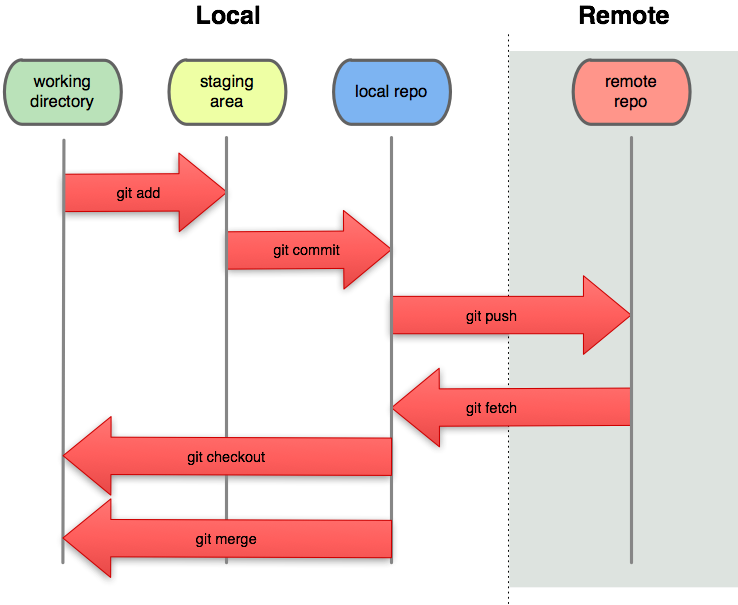
\includegraphics[width=0.8\textwidth]{Lecture2/git_workflow.png}
  \caption{}
  \label{fig:gitflow}
\end{center}
\end{figure}

\subsection*{What do I need to use Git?}

\begin{itemize}
\item A {\bf Git server} enabling multi-person collaboration through a centralized repository.
\item A {\bf Git client} on your own machine.

  \begin{itemize}
    \item Linux: Git client program is shipped with many Linux distributions, e.g., Ubuntu and CentOS. If not, install using a package manager, e.g., \colorbox{shadecolor}{yum install git} on CentOS.
    \item Mac: follow instructions at \href{https://www.atlassian.com/git/tutorials/install-git}{https://www.atlassian.com/git/tutorials/install-git}.
    \item Windows: Git for Windows at \href{https://gitforwindows.org}{https://gitforwindows.org} (GUI) aka Git Bash.
  \end{itemize}
\item Do {\bf not} totally rely on GUI or IDE. Learn to use Git on command line, which is needed for cluster and cloud computing.

\end{itemize}

\subsection*{Git survival commands}

\begin{itemize}
  \item \colorbox{shadecolor}{git pull} synchronize local Git directory with remote repository.
  \item Modify files in local working directory.
  \item \colorbox{shadecolor}{git add FILES} add snapshots to staging area
  \item \colorbox{shadecolor}{git commit -m ``message''} store snapshots permanently to ({\bf local}) Git repository
  \item \colorbox{shadecolor}{git push} push commits to remote repository.
\end{itemize}

\subsection*{Git basic usage}

Working with your local copy.

\begin{itemize}

    \item \colorbox{shadecolor}{git pull}: update local Git repository with remote repository (fetch + merge).
    
    \item \colorbox{shadecolor}{git log FILENAME}: display the current status of working directory.
    
    \item \colorbox{shadecolor}{git diff}: show differences (by default difference from the most recent commit). 
    
    \item \colorbox{shadecolor}{git add file1 file2 ...}: add file(s) to the staging area.
    
    \item \colorbox{shadecolor}{git commit}: commit changes in staging area to Git directory.
    
    \item \colorbox{shadecolor}{git push}: publish commits in local Git repository to remote repository.

    \item \colorbox{shadecolor}{git reset --soft HEAD~1}: undo the last commit. 

    \item \colorbox{shadecolor}{git checkout FILENAME}: go back to the last commit, discarding all changes made.
    
    \item \colorbox{shadecolor}{git rm FILENAME}: remove files from git control.
\end{itemize}


\newpage
\subsection*{Vector and vector space}

(from JM Appendix A)

\begin{itemize}
\item A set of vectors $\vecc{x}_1, \dots, \vecc{x}_n$ are {\it linearly dependent} if there exist coefficients $c_j$ for $j = 1, 2, \dots, n$ such that $\sum_{j=1}^{n}{c_j \vecc{x}_j} = \vecc{0}$ and $||\vecc{c}||_2 = \sum_{j=1}^{n}{c_j^2}>0$.
They are {\it linearly independent} if  $\sum_{j=1}^{n}{c_j \vecc{x}_j} = \vecc{0}$ implies $c_j = 0$ for all $j$.

\item Two vectors are {\it orthogonal} to each other, written $\vecc{x} \bot \vecc{y}$, if their inner product is 0, that is $\vecc{x}\transpose\vecc{y} = \vecc{y}\transpose\vecc{x} = \sum\limits_{j}{x_j y_j} = 0$.

\item A set of vectors $\vecc{x}^{(1)}, \vecc{x}^{(2)}, \dots, \vecc{x}^{(n)}$ are mutually orthogonal iff $\vecc{x}^{(i)T}\vecc{x}^{(j)} = 0$ for $\forall i \ne j$.

\item The most common set of vectors that are mutually orthogonal are the {\it elementary} vectors $\vecc{e}^{(1)}, \vecc{e}^{(2)}, \dots, \vecc{e}^{(n)}$, which are all zero, except for one element equal to $1$, so that $\vecc{e}^{(i)}_i = 1$ and $\vecc{e}^{(i)}_j = 0, \forall j \ne i$.

\item A {\it vector space} $\mathcal{S}$ is a set of vectors that are closed under addition and scalar multiplication, that is 

  \begin{itemize}
    \item if $\vecc{x}^{(1)}$ and $\vecc{x}^{(2)}$ are in $\mathcal{S}$, then $c_1 \vecc{x}^{(1)} + c_2 \vecc{x}^{(2)}$ is in $\mathcal{S}$.
  \end{itemize}

\item A vector space $\mathcal{S}$ is {\it generated} or {\it spanned} by a set of vectors $\vecc{x}^{(1)}, \vecc{x}^{(2)}, \dots, \vecc{x}^{(n)}$, written as $\mathcal{S} = \mbox{span}\{\vecc{x}^{(1)}, \vecc{x}^{(2)}, \dots, \vecc{x}^{(n)}\}$, 
if any vector $\vecc{x}$ in the vector space is a linear combination of $\vecc{x}_i, i=1, 2, \dots, n$.

\item A set of linearly independent vectors that generate or span a space $\mathcal{S}$ is called a {\it basis} of $\mathcal{S}$.

\end{itemize}

\subsubsection*{Example A.1}

Let
$$
\vecc{x}^{(1)} = \left[ \begin{array}{c} 1\\ 1\\ 1\\ 1\\ \end{array} \right], \vecc{x}^{(2)} = \left[ \begin{array}{c} 1\\ 2\\ 3\\ 4\\ \end{array} \right], \mbox{ and } \vecc{x}^{(3)} = \left[ \begin{array}{c} -3\\ -1\\ 1\\ 3\\ \end{array} \right].
$$

Then $\vecc{x}^{(1)}$ and $\vecc{x}^{(2)}$ are linearly independent, but $\vecc{x}^{(1)}$, $\vecc{x}^{(2)}$, and $\vecc{x}^{(3)}$ are linearly dependent since $5\vecc{x}^{(1)} - 2\vecc{x}^{(2)} + \vecc{x}^{(3)} = 0$


\subsection*{Rank}

Some matrix concepts arise from viewing columns or rows of the matrix as vectors.  Assume $\vecc{A} \in \mathbb{R}^{m \times n}$.

\begin{itemize}
\item $\rank(\vecc{A})$ is the maximum number of linearly independent rows or columns of a matrix.

\item $\rank(\vecc{A}) \le \min\{m, n\}$.

\item A matrix is {\it full} rank if $\rank(\vecc{A}) = \min\{m, n\}$.  It is {\it full row rank} if $\rank(\vecc{A}) = m$.  It is {\it full column rank} if $\rank(\vecc{A}) = n$.

\item a square matrix $\vecc{A} \in \mathbb{R}^{n \times n}$ is {\it singular} if $\rank(\vecc{A}) < n$ and {\it non-singular} if $\rank(\vecc{A}) = n$.

\item $\rank(\vecc{A}) = \rank(\vecc{A}\transpose) = \rank(\vecc{A}\transpose\vecc{A}) = \rank(\vecc{A}\vecc{A}\transpose)$. (Show this in HW.)

\item $\rank(\vecc{A}\vecc{B}) \le \min\{\rank(\vecc{A}), \rank(\vecc{B})\}$. (Hint: Columns of $\vecc{A}\vecc{B}$ are spanned by columns of A and rows of of $\vecc{A}\vecc{B}$ are spanned by rows of B.)

\item if $\vecc{Ax} = \vecc{0}_m$ for some $\vecc{x} \ne \vecc{0}_n$, then $\rank(\vecc{A}) \le n - 1$.

\end{itemize}